%!TEX root = ./Consignes_Rapport_Technique.tex

\begin{appendix}
\section{Annexe spécifique a HLM509}

\subsection{Contours des projets}

\subsubsection{Objectifs}
Les objectifs principaux des PIM sont:
\begin{itemize}
\item Un premier contact avec la démarche de modélisation qui est de plus en plus présente dans les bureaux d’études \\ \ \\
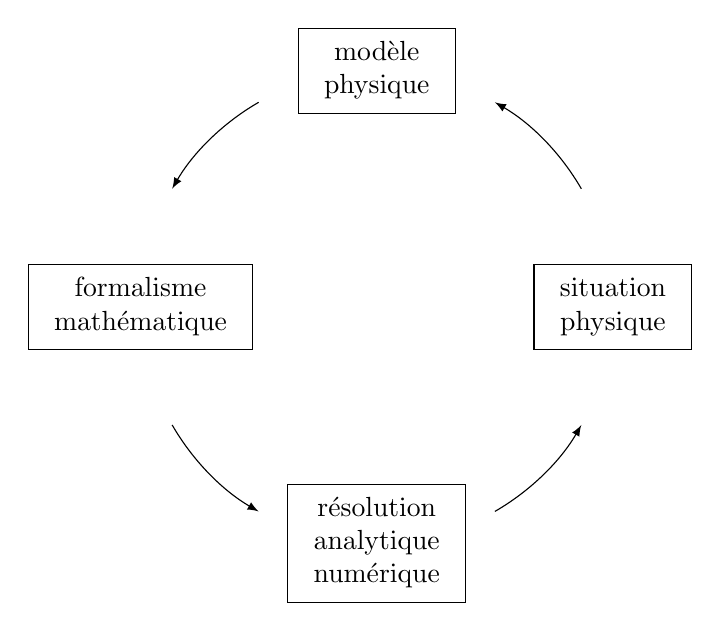
\begin{tikzpicture}

\def \radius {3cm}
\def \margin {30} % margin in angles, depends on the radius
  \node[draw, rectangle] at ({360/4 * (1 - 1)}:\radius) {\begin{tabular}{c}situation\\physique\end{tabular}};
  \draw[->, >=latex] ({360/4 * (1 - 1)+\margin}:\radius) 
    arc ({360/4 * (1 - 1)+\margin}:{360/4 * (1)-\margin}:\radius);
%
  \node[draw, rectangle] at ({360/4 * (2 - 1)}:\radius) {\begin{tabular}{c}modèle\\physique\end{tabular}};
  \draw[->, >=latex] ({360/4 * (2 - 1)+\margin}:\radius) 
    arc ({360/4 * (2 - 1)+\margin}:{360/4 * (2)-\margin}:\radius);
%
  \node[draw, rectangle] at ({360/4 * (3 - 1)}:\radius) {\begin{tabular}{c}formalisme\\mathématique\end{tabular}};
  \draw[->, >=latex] ({360/4 * (3 - 1)+\margin}:\radius) 
    arc ({360/4 * (3 - 1)+\margin}:{360/4 * (3)-\margin}:\radius);
%
  \node[draw, rectangle] at ({360/4 * (4 - 1)}:\radius) {\begin{tabular}{c}résolution\\analytique\\numérique\end{tabular}};
  \draw[->, >=latex] ({360/4 * (4 - 1)+\margin}:\radius) 
    arc ({360/4 * (4 - 1)+\margin}:{360/4 * (4)-\margin}:\radius);
%
\end{tikzpicture}

\item Apprendre différemment
\end{itemize}

\subsubsection{Règles du jeu}
Pour l'essentiel les Projets numériques consistent en:
\begin{itemize}
\item 1 groupe + 1 tuteur + 1 sujet
\item un sujet ouvert
\item un tuteur expert
\item des heures de consultation
\item un point de vue opposé d’un cours magistral: il faut demander pour recevoir
\end{itemize}

\subsubsection{Quelques dates}
\begin{itemize}
\item Début semestre d'année : constitution des groupes et attribution des sujets
\item Mi Semestre : remise du premier document et présentations des premiers résultats 
\item Fin du semestre : remise du rapport (15-20 pages) et soutenance orale
\end{itemize}


\subsubsection{Quelques pièges à éviter}
\begin{itemize}
\item travail d'équipe
\item gestion du temps ... et du stress 
\item le temps des notes faciles est révolu
\item Notation mixte globale/individuelle
	\begin{itemize}
	\item 1/3 : rapport (double correction)
	\item 1/3 : présentation (jury)
	\item 1/3 : travail (tuteur) + soutenance de mi-parcours
	\end{itemize}
\end{itemize}


\subsubsection{Grille d'évaluation}
Les points suivants sont évalués en priorité:
\begin{itemize}
\item Description du contexte, motivation et objectif de l’étude
\item Présentation des hypothèses de travail, écriture du modèle physique
\item Compréhension de la méthode de résolution
\item Analyse critique/physique des résultats obtenus. Retour éventuel sur les hypothèses
\item Qualité de la forme: figure, orthographe, précision du langage
\end{itemize}

\subsection{Conseils pour la présentation orale des projets}

\subsubsection{Conseils généraux}
\begin{itemize}
\item La "star" c’est vous, pas l’écran
\item Soyez clair, quitte à simplifier votre discours en ne discutant pas tous les détails: pour être appréciée, une présentation doit d’abord être comprise par le public
\item Ne pas montrer ce que l’on ne présente pas. Le matériel est soit indispensable et on en parle, soit inutile et on ne le montre pas
\item Parler suffisamment fort, et regarder votre public
\item Numéroter les planches, respecter le temps imparti, répéter
\item Pour vérifier que votre support de présentation oral est adapté (taille des caractères, couleurs, contraste): allez en salle SC001, projeter vos slides et mettez vous au fond de la salle. Si vous ne voyez pas l’ensemble des informations écrites, ce n’est pas bon !
\end{itemize}

\subsubsection{Introduction}
\begin{itemize}
\item Partie cruciale de l’exposé: doit être comprise par tous. Entre 10 et 30\% de l’exposé pour bien motiver l’étude
\item Elle doit répondre aux questions suivantes :
\item Quel est le contexte industriel ? Scientifique ?
\item Quels sont les phénomènes mis en jeu dans le problème ?
\item Que faut-il étudier ? Pourquoi ? Quelles quantités intéressantes ?
\item Qu’est-ce que votre étude peut apporter ?
\item Mettre des photos, des films, des schémas : des images !
\end{itemize}

\subsubsection{Présentation du problème}
\begin{itemize}
\item Rappeler les hypothèses de travail
\item Mettre des schémas de la configuration étudiée
\item Ne pas surcharger d’équations
\item "Faire parler" les équations: expliciter les termes, dire à quelle physique ils correspondent. Lire uniquement les équations à haute voix ne sert à rien.
\end{itemize}

\subsubsection{Présentation des résultats - Figures}
\begin{itemize}
\item Mettre des axes avec des unités, des légendes
\item Mettre des traits épais, des couleurs vives (pas de jaune, vert clair etc)
\item Les légendes/labels/titres/traits doivent être \textbf{très} gros
\item Les figures des présentations ne sont pas les mêmes que ceux des rapports: \textbf{chaque figure doit être faite deux fois}
\item Comparaison deux 2 courbes : les mettre sur le même graphe ou tracer la différence
\item Comparaison de champs 2D: utiliser les mêmes échelles de couleur ou tracer la différence
\item Pour les problèmes instationnaires, les films sont à privilégier
\end{itemize}

\end{appendix}
